\documentclass[a4paper, 12pt]{article}
\usepackage[T2A]{fontenc}
\usepackage[utf8]{inputenc}
\usepackage[english,russian]{babel}
\usepackage{amsmath, amsfonts, amssymb, amsthm, mathtools, misccorr, indentfirst, multirow}
\usepackage{wrapfig}
\usepackage{graphicx}
\usepackage{subfig}
\usepackage{adjustbox}
\usepackage{pgfplots}

\usepackage{geometry}
\geometry{top=20mm}
\geometry{bottom=20mm}
\geometry{left=20mm}
\geometry{right=20mm}
\newcommand{\angstrom}{\textup{\AA}}
\begin{document}
	\begin{titlepage}
		\begin{center}
		МИНИСТЕРСТВО ОБРАЗОВАНИЯ И НАУКИ РОССИЙСКОЙ ФЕДЕРАЦИИ\\
		\footnotesize{Московский физико-технический институт}\\
		\footnotesize{(государственный университет)}\\
		\footnotesize{Кафедра вакуумной электроники}\\
		\vfill
		{\LARGE
		\textbf{Автоэлектронная эмиссия}\\
		}
		\vspace{1cm}
		Лабораторная работа по курсу\\
		вакуумная электроника
		\vfill
		\begin{flushright}
			Выполнил: студент 654гр.\\
			Нехаев А.С.
		\end{flushright}
		\vfill
		г. Долгопрудный\\
		2018 год
		\end{center}
	\end{titlepage}
	\newpage
	\pagenumbering{arabic}
	\tableofcontents
	\newpage
	\section{Цель работы}
	\begin{enumerate}
		\item Изучить особенности автоэлектронной эмиссии и её применения.
		\item Ознакомиться с техникой автоэлектронной микроскопии и областями её применения, а также методикой получения острий для автоэмиссионных микроскопов.
		\item Исследовать автоэмиссионные свойства катода из углеродных волокон и причины нестабильности автоэмиссионного тока в нем.
	\end{enumerate}
	\newpage
	\section{Теоретическая часть}
	Автоэлектронная эмиссия - это явление испускания электронов в вакуум под воздействием сильного электрического поля порядка $10^7$ В/см с поверхности твердого поля. Для уменьшения необходимого напряжения катоду придают форму тонкого острия. Суть явления состоит в туннелировании электронов сквозь потенциальный барьер в результате его искривления под воздействием электрического поля.\par
	Для нахождения плотности тока автоэлектронной эмиссии используется формула Фаулера-Нордгейма
	\begin{equation}
		j=\frac{A'E^2}{\varphi}\cdot e^{-\frac{B'\cdot \varphi^{\frac{3}{2}}}{E}},	
	\end{equation}
	где $A'=\frac{e^3}{8\pi h}e^{0.739\cdot\frac{\frac{8\pi}{3e}\left(2m\varphi^3\right)^{\frac{1}{2}}}{hE}}$, $B'=0.965\cdot\frac{\frac{8\pi}{3e}\left(2m\varphi^3\right)^{\frac{1}{2}}}{hE}$. Эта формула выведена для $T=0$, но так как при комнатной температуре $\varphi\gg kT$ применима и в нашем случае. Также, построив ВАХ в координатах Фаулера-Нордгейма возможно вычислить форм-фактор катода по формуле
	\begin{equation}
		\tan(\alpha)=-0.683\cdot\frac{\varphi^{\frac{3}{2}}}{\beta},
	\end{equation}
	где $\alpha$ -- угол наклона получившейся кривой. Основными механизмами нестабильности автоэлектронной эмиссии являются: разрушение поверхности катода ионами остаточных газов, абсорбция и десорбция атомов остаточных газов, разрушение катода пондеромоторными силами, смещение элементов катода за счет электростатического отталкивания.
	\section{Техника эксперимента}
	В качестве катода выступал пучок углеродных волокон, стравленный предварительно коронным разрядом, в результате электрическое поле для всех волокон пучка было почти одинаковым. Исследуемые автокатоды находились в отпаянной стеклянной лампе. На анод подавалось высокое напряжение, а катод заземлялся.
	\newpage
	\section{Практическая часть}
	\begin{enumerate}
		\item Сняли зависимость автоэмиссионного тока катода из углеродных трубок от приложенного напряжения
		\begin{figure}[!htb]
			\centering
			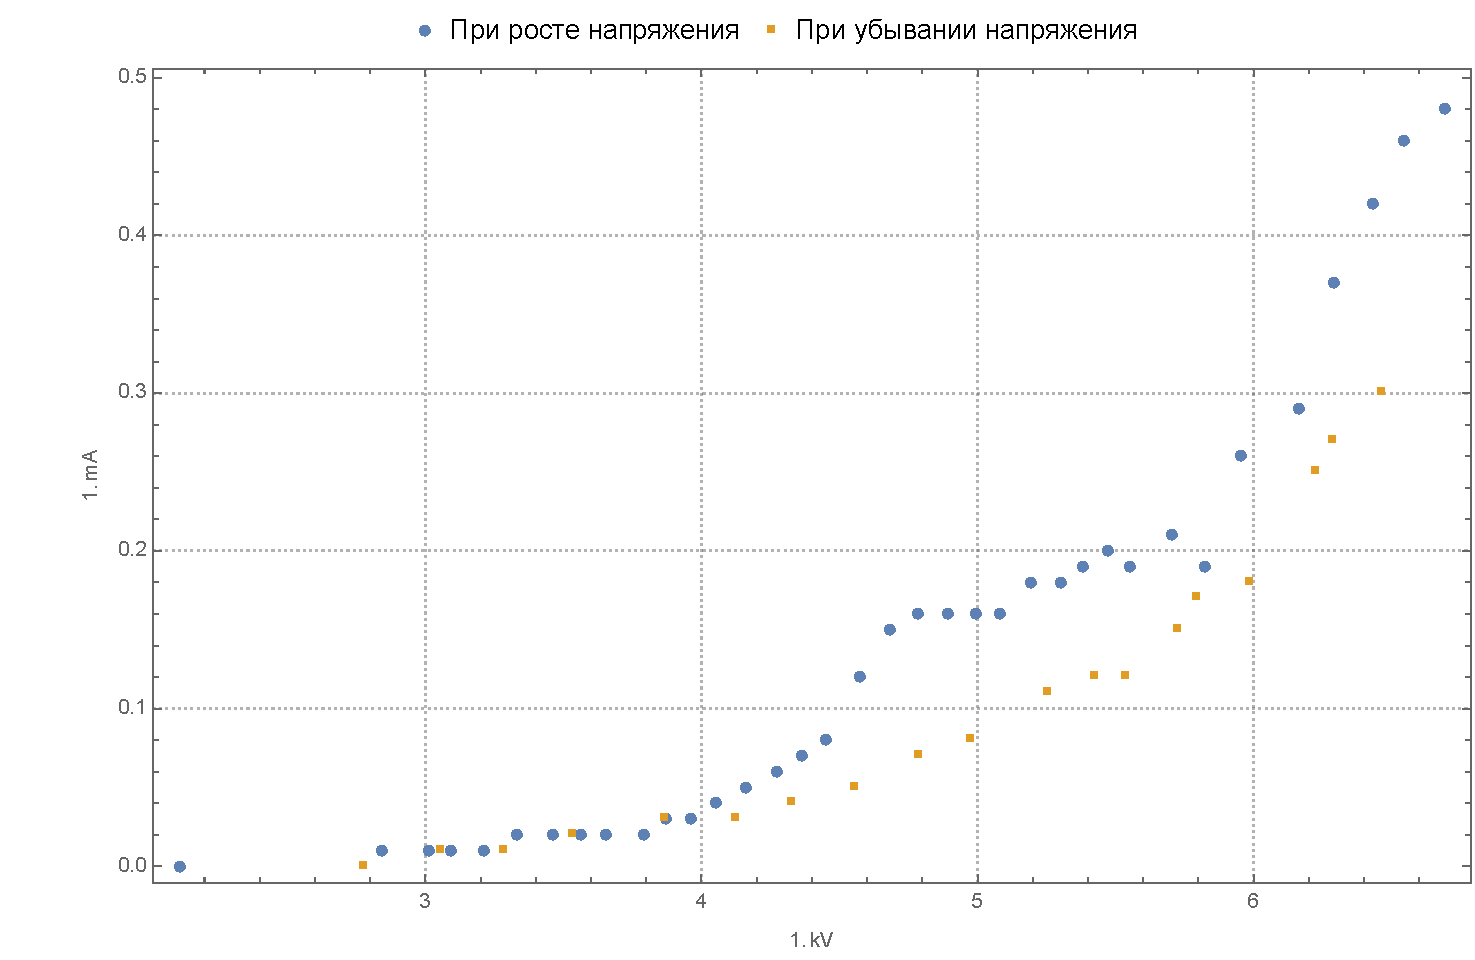
\includegraphics[scale=0.5]{fig1.pdf}
			\caption{График зависимости автоэмиссионного тока от напряжения}
		\end{figure}
		\\
		По графику можно определить, что ВАХ системы отличалась при возрастании и убывании напряжения.
		\item Построили полученную зависимость в координатах Фаулера-Нордгейма
		\begin{figure}[!htb]
			\centering
			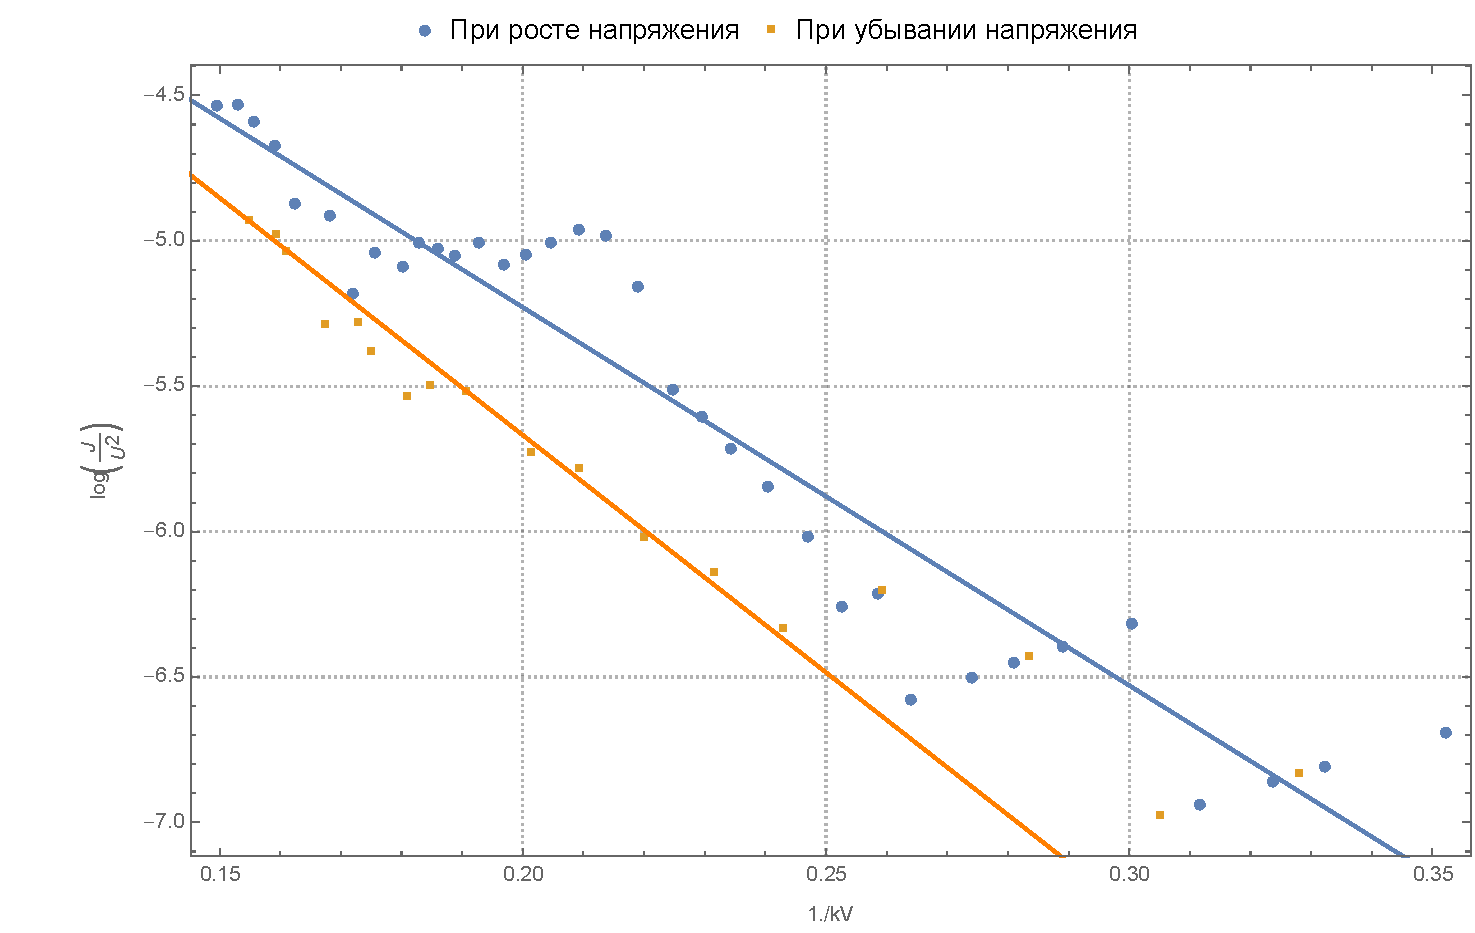
\includegraphics[scale=0.55]{fig2.pdf}
			\caption{График зависимости давления от времени}
		\end{figure}\\
		По полученным кривым можно выяснить, что основную роль в нестабильности тока имело изменение размеров эмиссионных центров, так как значение величины А + 2ln(B), где А – смещение кривой ФН, а B - её коэффициент наклона, осталось почти постоянным в  течение снятия ВАХ.\par
		Форм фактор для возрастания и убывания соответственно равен $\beta=-\frac{0.683\varphi^{\frac{3}{2}}}{\tan(\alpha)}$
	\end{enumerate}
	\newpage
	\section{Вывод}
	\begin{enumerate}
		\item Изучили особенности автоэлектронной эмиссии и её применения.
		\item Ознакомились с техникой автоэлектронной микроскопии и областями её применения, а также методикой получения острий для автоэмиссионных микроскопов
		\item Исследовали автоэмиссионные свойства катода из углеродных волокон и определили причину нестабильности автоэмиссионного тока такого катода.
	\end{enumerate}
\end{document}